\documentclass[11pt,a4paper]{article}

\usepackage[utf8]{inputenc}
\usepackage[T1]{fontenc}
\usepackage{lmodern}
\usepackage[margin=1in]{geometry}
\usepackage{amsmath,amssymb,amsfonts}
\usepackage{booktabs}
\usepackage{graphicx}
\usepackage{float}
\usepackage{hyperref}
\usepackage{caption}
\usepackage{subcaption}

\hypersetup{
    colorlinks=true,
    linkcolor=blue,
    urlcolor=blue,
    citecolor=blue
}

\title{\textbf{Reverse-Engineering Gene Regulatory Networks\\Using Dynamic Bayesian Networks}}
\author{\textbf{Pavel Charheika}\\Faculty of Mathematics, Informatics, and Mechanics\\University of Warsaw}
\date{}

\begin{document}

\maketitle

\begin{abstract}
This study evaluates the efficacy of Dynamic Bayesian Networks (DBNs) in reconstructing the structure of Gene Regulatory Networks (GRNs) from discrete time-series expression data. Utilizing the exact structure-learning algorithm implemented in \texttt{BNFinder2}, we investigate the impact of network size, update dynamics (synchronous vs.\ asynchronous), temporal sampling frequency, and scoring criteria (Minimum Description Length vs.\ Bayesian-Dirichlet Equivalence) across both synthetic Random Boolean Networks ($N \in \{5, 8, 10, 13, 16\}$) and the 10-node Mammalian Cell Cycle biological network. Empirical results demonstrate that synchronous and transient pre-attractor trajectories consistently yield the highest precision (up to $1.00$ on synthetic topologies and $0.82$ on the biological network) and lowest Structural Hamming Distance ($\text{SHD} = 24$).
\end{abstract}

\section{Introduction}
Reconstructing causal regulatory interactions from time-series gene expression profiles is a central inverse problem in computational systems biology. Dynamic Bayesian Networks (DBNs) model temporal stochastic processes by restricting directed edges to point strictly forward in time ($t \to t+1$), thereby unrolling cyclic feedback loops into a bipartite Directed Acyclic Graph (DAG) and enabling exact polynomial-time parent set identification.

The study is structured in two experimental phases:
\begin{enumerate}
    \item \textbf{Part I (Synthetic Topology Benchmark):} Systematic evaluation on Random Boolean Networks (RBNs) of increasing size ($N \in \{5, 8, 10, 13, 16\}$ nodes, in-degree $k \in \{1, 2, 3\}$) across four distinct dynamical regimes.
    \item \textbf{Part II (Biological Network Reconstruction):} Validation on the 10-node Mammalian Cell Cycle network compiled from Boolean rules (\texttt{.bnet}) into exact truth tables.
\end{enumerate}

\section{Mathematical Formulation \& Methodology}

\subsection{Dynamic Bayesian Network Structure Learning}
Let $\mathbf{X}^{(t)} = (X_1^{(t)}, \dots, X_n^{(t)}) \in \{0, 1\}^n$ denote the binary expression state vector at discrete time step $t$. Under the first-order Markov assumption, the transition probability factorizes over a graph $\mathcal{G} = (\mathcal{V}, \mathcal{E})$:
\begin{equation}
P\left(\mathbf{X}^{(t+1)} \mid \mathbf{X}^{(t)}, \mathcal{G}, \Theta\right) = \prod_{i=1}^{n} P\left(X_i^{(t+1)} \mid \mathbf{Pa}_i^{(t)}, \theta_i\right)
\end{equation}
where $\mathbf{Pa}_i^{(t)} \subseteq \mathbf{X}^{(t)}$ denotes the regulator parent set of node $X_i$. Given $N$ observed transitions $\mathcal{D}$, we compare two decomposable scoring functions in \texttt{BNFinder2}:
\begin{itemize}
    \item \textbf{Minimum Description Length (MDL):} Penalizes model complexity (parent set cardinality) to enforce parsimony and suppress spurious edges:
    \begin{equation}
    \text{MDL}(X_i, \mathbf{Pa}_i : \mathcal{D}) = -\sum_{j=1}^{q_i} \sum_{k \in \{0,1\}} N_{ijk} \log_2 \left( \frac{N_{ijk}}{N_{ij}} \right) + \frac{\log_2 N}{2} q_i (r_i - 1)
    \end{equation}
    where $r_i = 2$, $q_i = 2^{|\mathbf{Pa}_i|}$, and $N_{ijk}$ is the transition count from parent configuration $j$ to child state $k$.
    \item \textbf{Bayesian-Dirichlet Equivalence (BDE):} Evaluates the marginal likelihood over a Dirichlet prior on transition parameters.
\end{itemize}

\subsection{Simulation Regimes}
To evaluate sensitivity to experimental conditions, four time-series regimes were simulated:
\begin{itemize}
    \item \textbf{Sync Base (\texttt{sync\_base}):} Deterministic simultaneous updates ($T = 100, \Delta t = 1$), representing noise-free trajectories.
    \item \textbf{Async (\texttt{async}):} Stochastic single-node updates per step ($T = 200, \Delta t = 1$), modeling biological update stochasticity.
    \item \textbf{Sampled (\texttt{sampled}):} Synchronous updates sub-sampled every 3rd step ($T = 150, \Delta t = 3$), modeling low temporal resolution.
    \item \textbf{Transient (\texttt{transient}):} Short synchronous bursts ($T = 20, \Delta t = 1$), capturing dynamic transitions prior to attractor convergence.
\end{itemize}

\section{Part I: Synthetic Network Analysis}

Table~\ref{tab:part1} and Figures~\ref{fig:p1_f1}--\ref{fig:p1_rec} summarize reconstruction performance across network sizes $N \in \{5, 8, 10, 13, 16\}$ (fixed random seed $42$).

\begin{itemize}
    \item \textbf{Topology \& Attractor Sensitivity:} Reconstruction accuracy depends heavily on attractor basin structure rather than node count alone. For $N = 5$, deterministic synchronous trajectories (\texttt{sync\_base} and \texttt{transient}) rapidly converged to a fixed point, providing insufficient state transitions for MDL/BDE ($F_1 = 0.00$), whereas stochastic \texttt{async} perturbations escaped the attractor and achieved $F_1 = 0.29$ ($\text{Precision} = 0.67$). Conversely, at $N = 10$, \texttt{sync\_base} and \texttt{transient} achieved strong recovery ($F_1 = 0.41, \text{Precision} = 0.86$ and $F_1 = 0.34, \text{Precision} = 0.71$, respectively).
    \item \textbf{Precision vs.\ Recall Bottleneck:} Across medium-to-large networks ($N \in \{10, 13, 16\}$), \texttt{sync\_base} and \texttt{transient} regimes maintain high precision (up to $1.00$ at $N = 13$), whereas recall drops sharply ($0.04 - 0.27$) as exponentially growing parent state combinations remain unobserved in a single trajectory.
    \item \textbf{Degradation under Sub-Sampling:} Recording every 3rd step (\texttt{sampled}) completely destroys the first-order Markov signal for $N \in \{5, 8, 10, 13\}$ ($F_1 = 0.00$) and yields only $F_1 = 0.06$ at $N = 16$.
\end{itemize}

\begin{figure}[H]
    \centering
    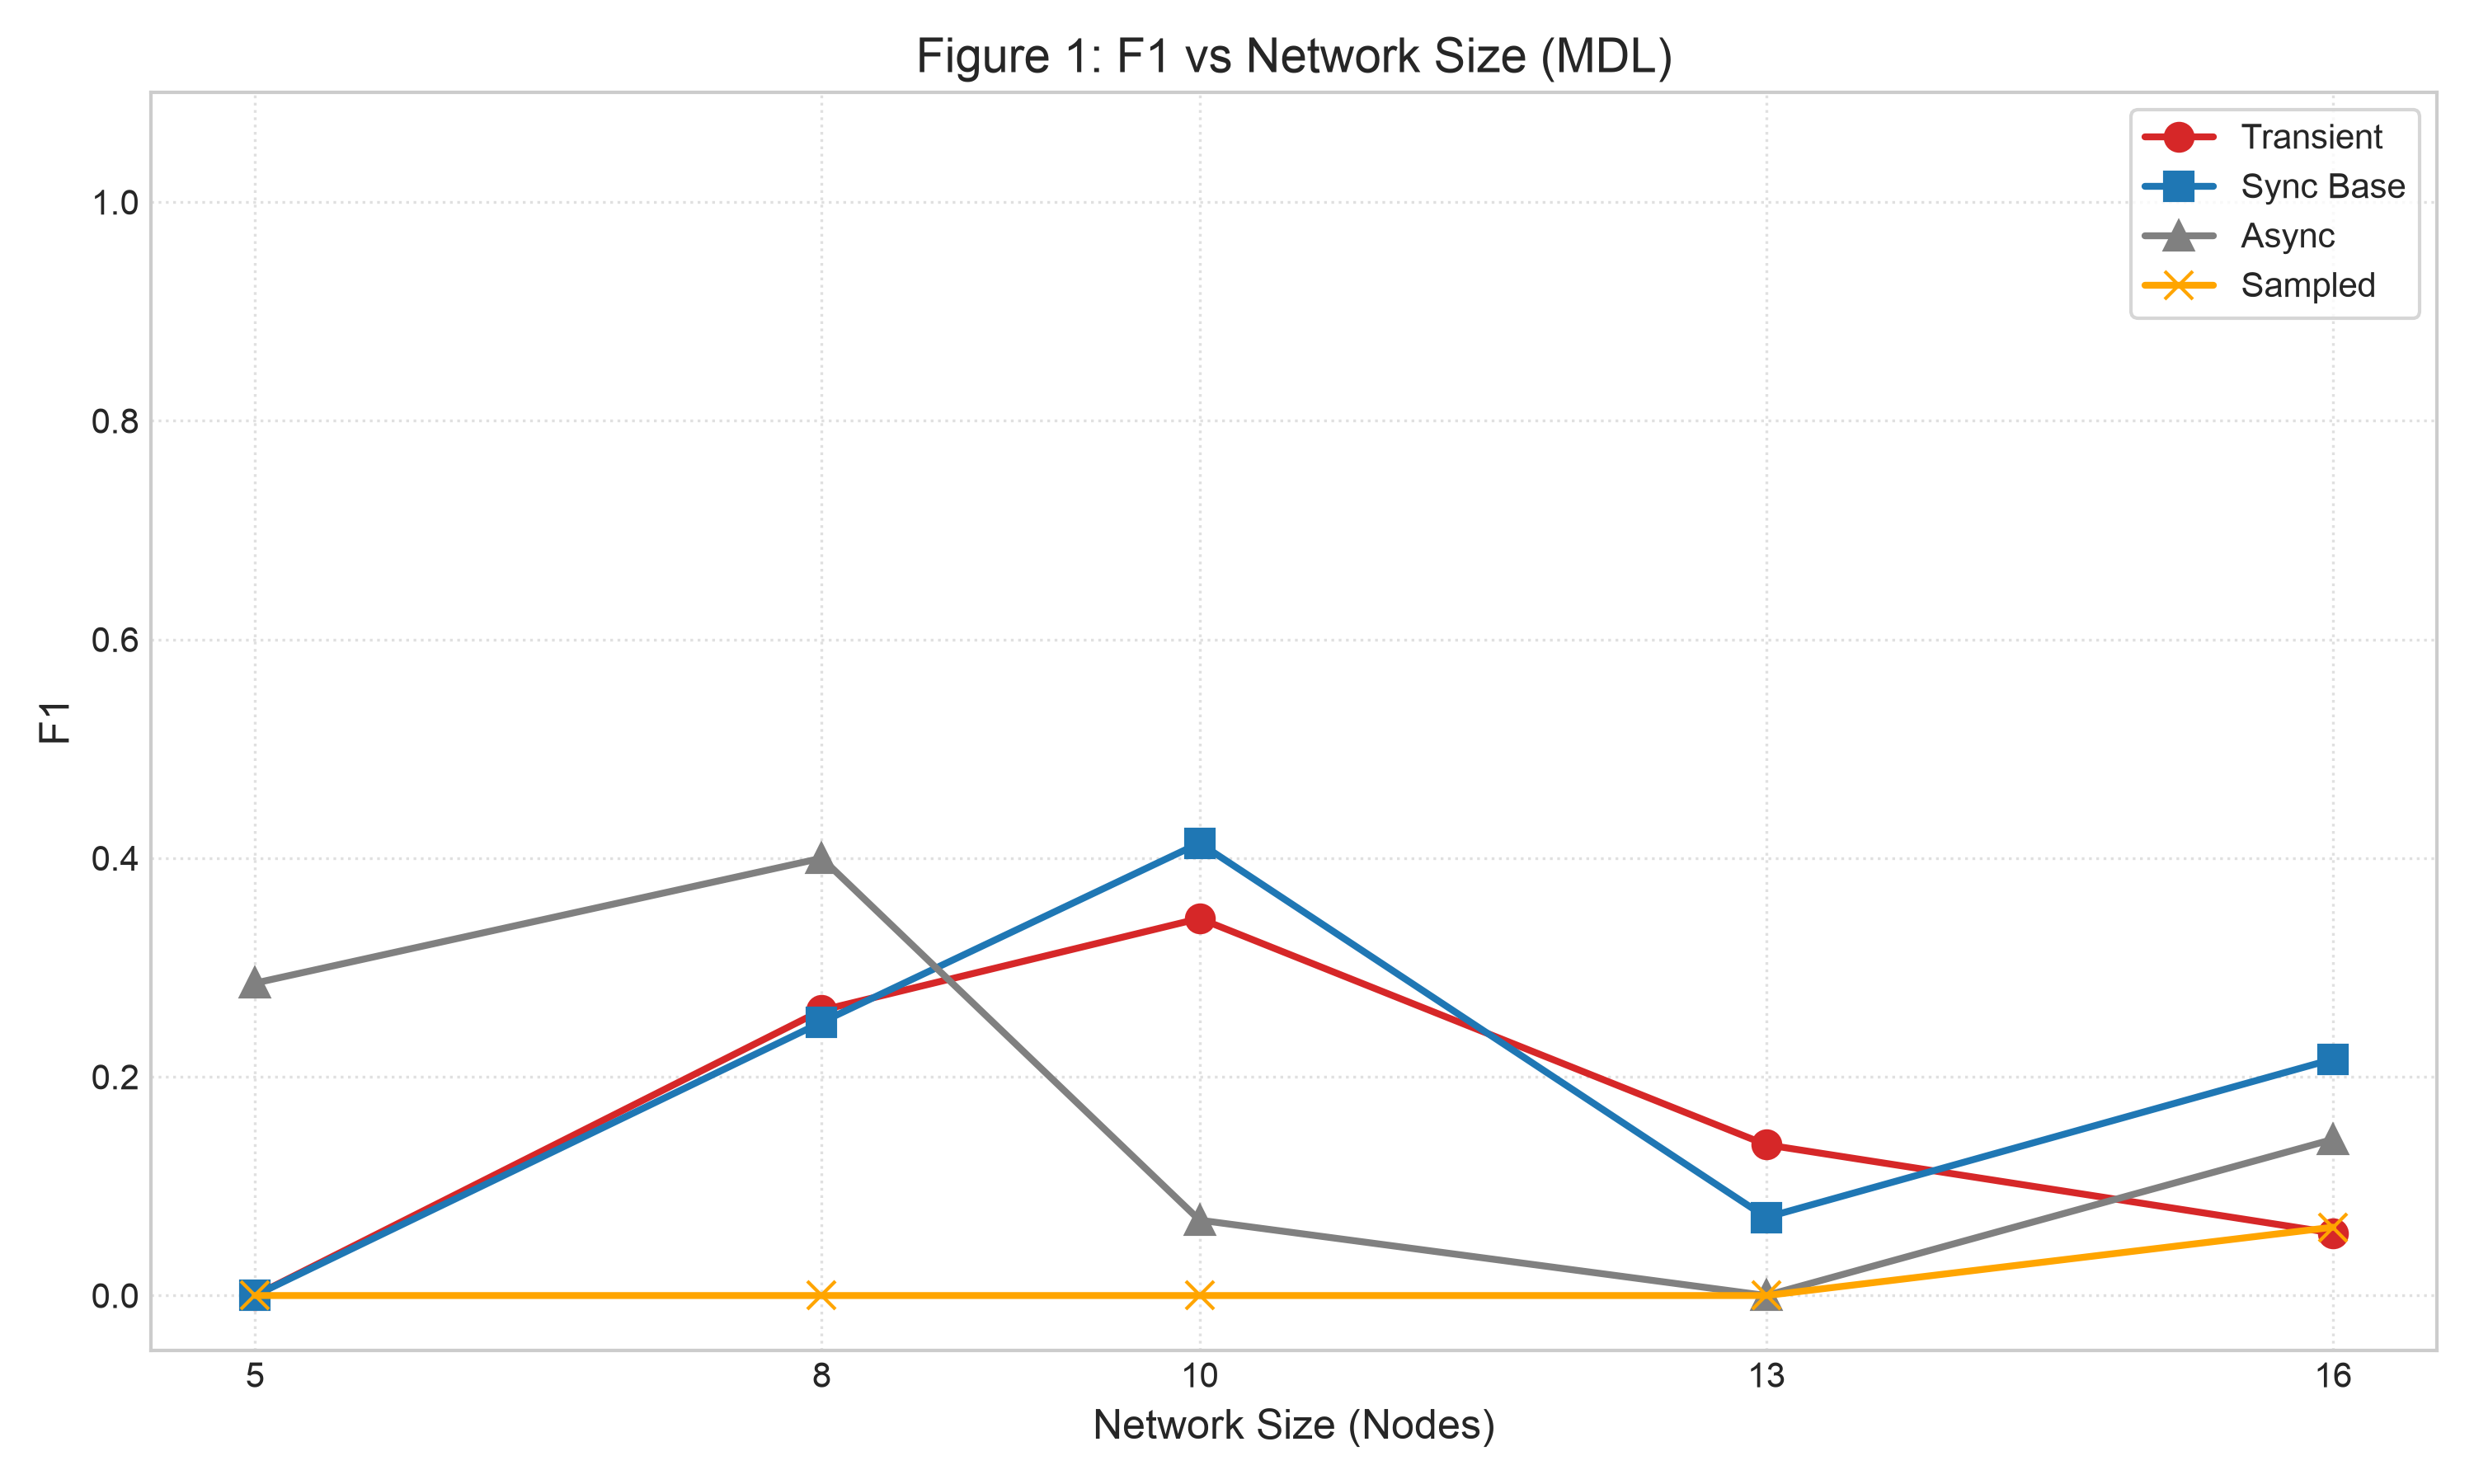
\includegraphics[width=0.78\textwidth]{../assets/part1_f1.png}
    \caption{Part I: Reconstruction $F_1$ Score vs.\ Network Size under MDL scoring.}
    \label{fig:p1_f1}
\end{figure}

\begin{figure}[H]
    \centering
    \begin{subfigure}[b]{0.48\textwidth}
        \centering
        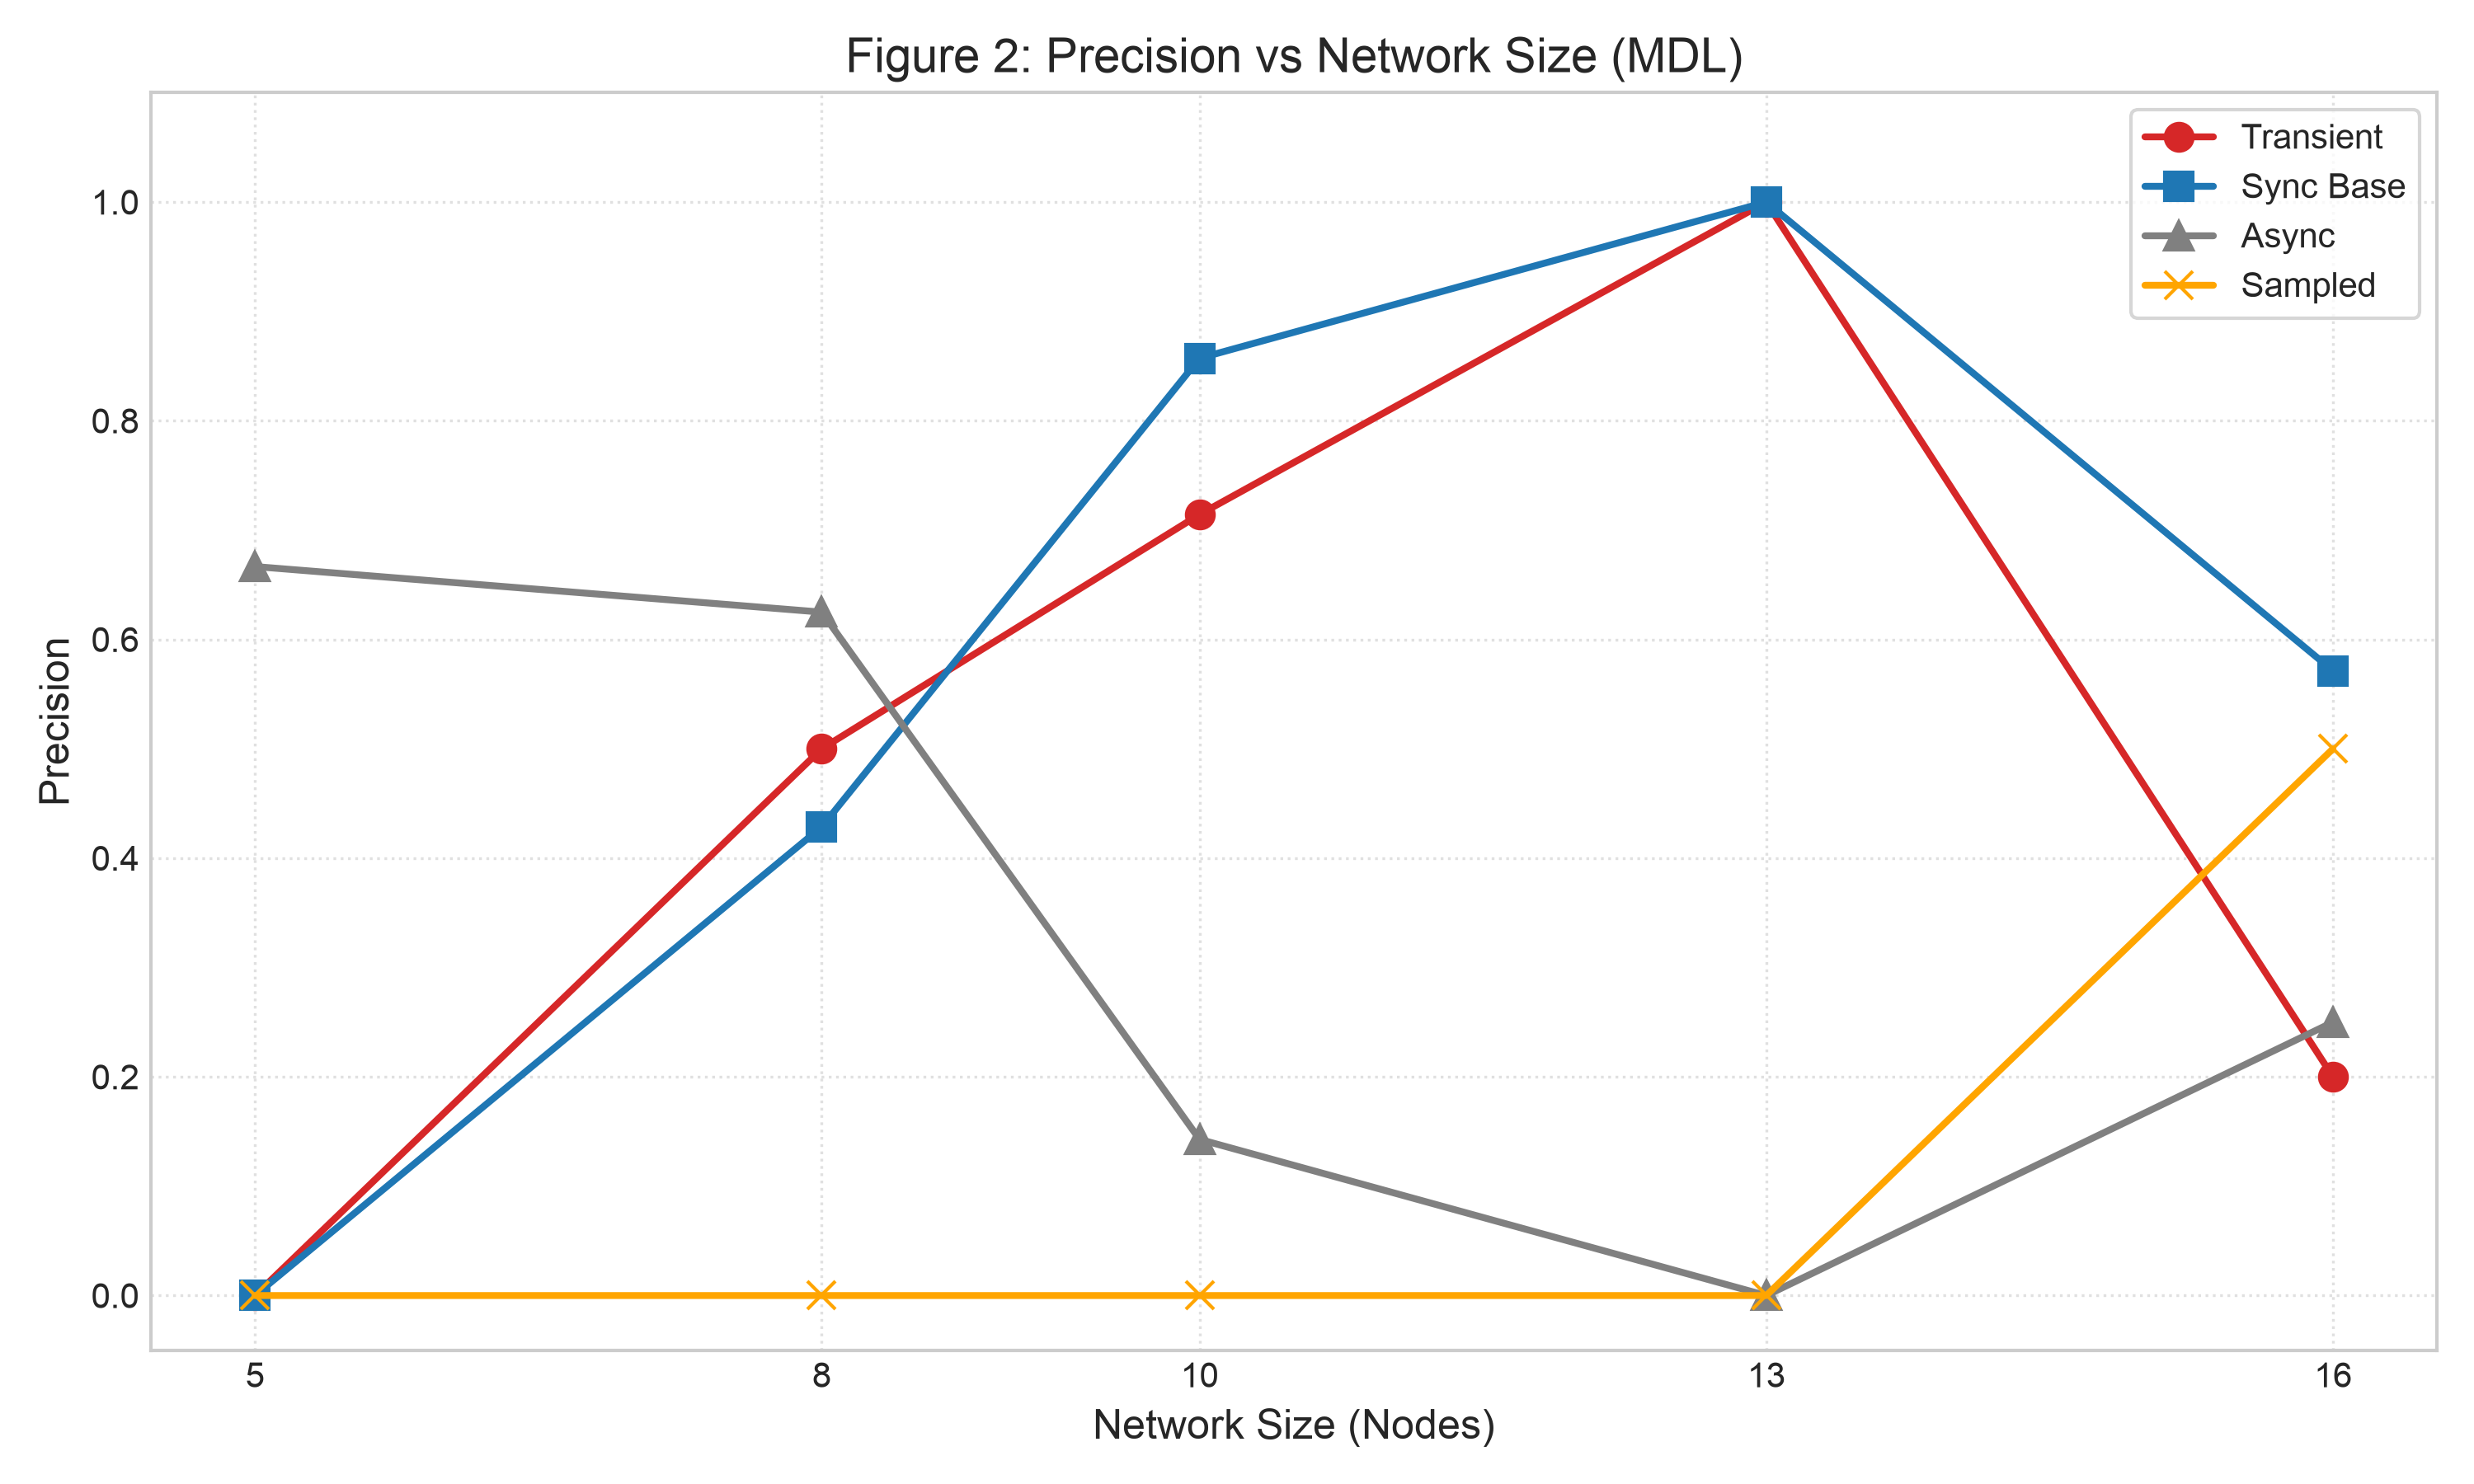
\includegraphics[width=\textwidth]{../assets/part1_precision.png}
        \caption{Precision vs.\ Network Size (MDL)}
        \label{fig:p1_prec}
    \end{subfigure}
    \hfill
    \begin{subfigure}[b]{0.48\textwidth}
        \centering
        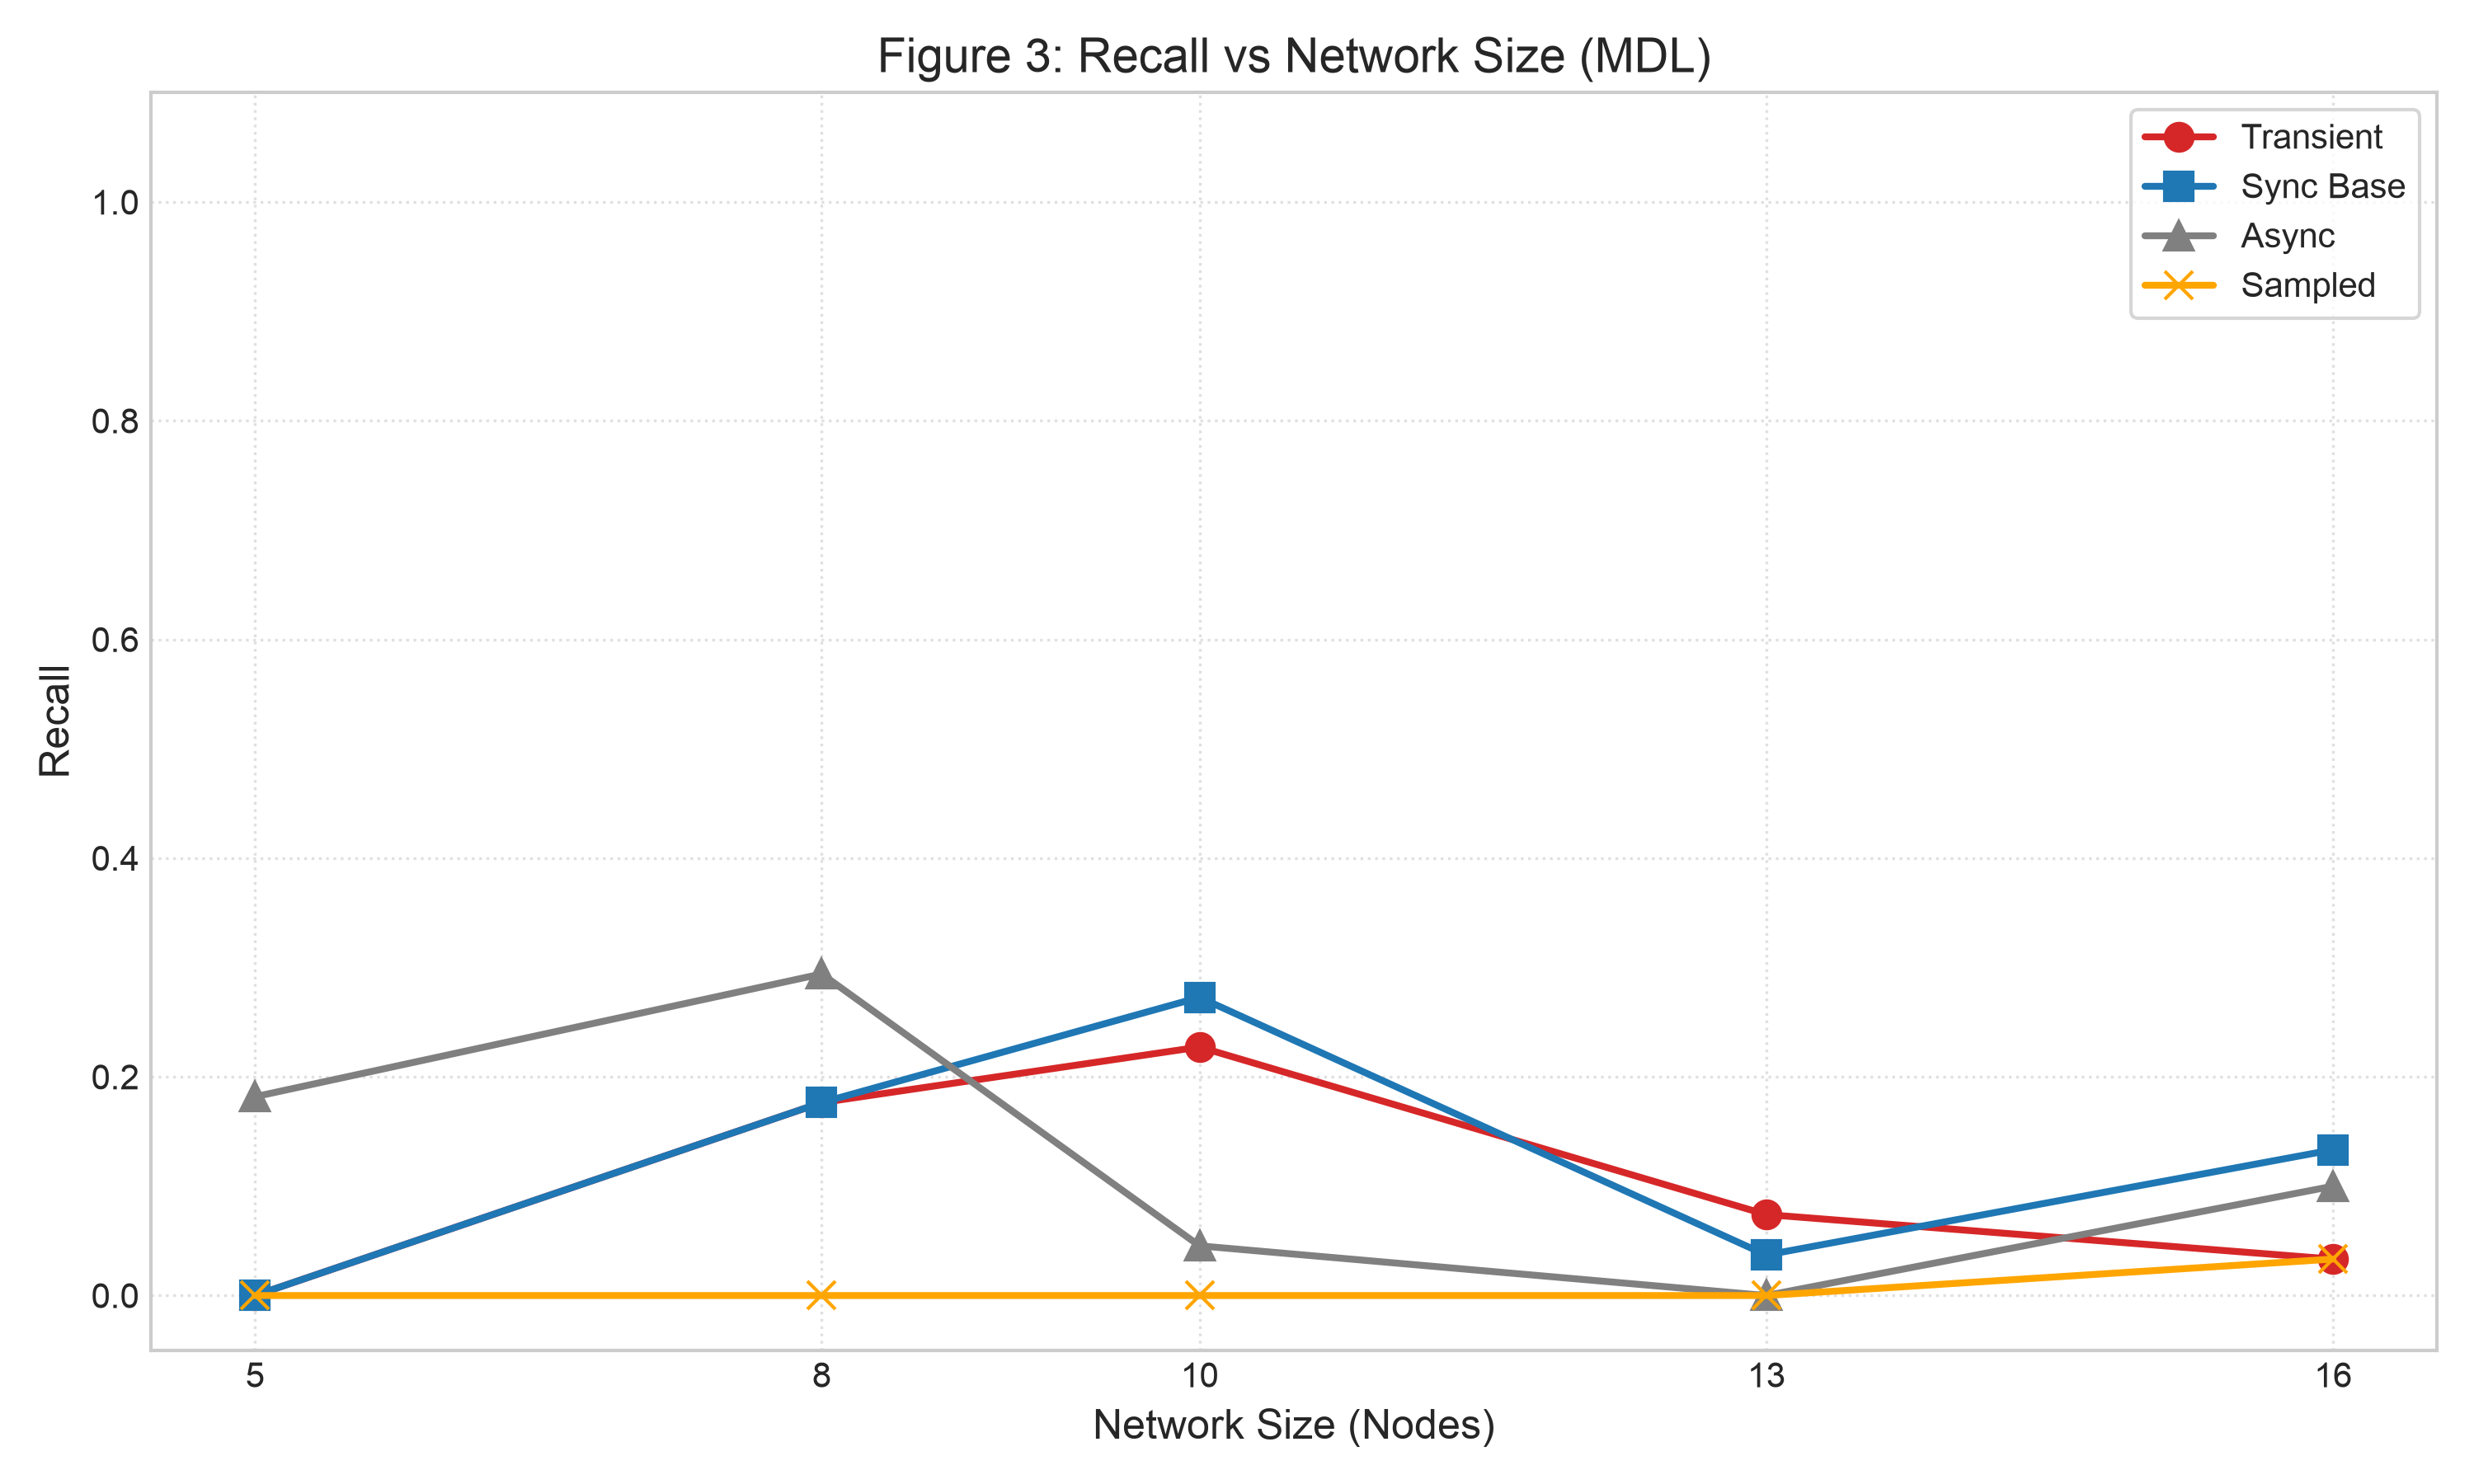
\includegraphics[width=\textwidth]{../assets/part1_recall.png}
        \caption{Recall vs.\ Network Size (MDL)}
        \label{fig:p1_rec}
    \end{subfigure}
    \caption{Decomposition of edge recovery into Precision and Recall across synthetic RBNs.}
\end{figure}

\begin{table}[H]
\centering
\caption{Part I Empirical Results: Synthetic Random Boolean Networks ($N \in \{5, 8, 10, 13, 16\}$).}
\label{tab:part1}
\small
\begin{tabular}{llcccc|llcccc}
\toprule
\textbf{Dataset} & \textbf{Meth} & \textbf{Prec} & \textbf{Rec} & \textbf{F1} & \textbf{SHD} & \textbf{Dataset} & \textbf{Meth} & \textbf{Prec} & \textbf{Rec} & \textbf{F1} & \textbf{SHD} \\
\midrule
\texttt{data\_5\_sync\_base}  & MDL & 0.00 & 0.00 & 0.00 & 11 & \texttt{data\_10\_sampled}    & MDL & 0.00 & 0.00 & 0.00 & 22 \\
\texttt{data\_5\_sync\_base}  & BDE & 0.00 & 0.00 & 0.00 & 11 & \texttt{data\_10\_sampled}    & BDE & 0.00 & 0.00 & 0.00 & 22 \\
\texttt{data\_5\_async}       & MDL & 0.67 & 0.18 & 0.29 & 10 & \texttt{data\_10\_transient}  & MDL & 0.71 & 0.23 & 0.34 & 19 \\
\texttt{data\_5\_async}       & BDE & 0.50 & 0.09 & 0.15 & 11 & \texttt{data\_10\_transient}  & BDE & 0.43 & 0.14 & 0.21 & 23 \\
\texttt{data\_5\_sampled}     & MDL & 0.00 & 0.00 & 0.00 & 11 & \texttt{data\_13\_sync\_base} & MDL & 1.00 & 0.04 & 0.07 & 26 \\
\texttt{data\_5\_sampled}     & BDE & 0.00 & 0.00 & 0.00 & 11 & \texttt{data\_13\_sync\_base} & BDE & 0.00 & 0.00 & 0.00 & 27 \\
\texttt{data\_5\_transient}   & MDL & 0.00 & 0.00 & 0.00 & 11 & \texttt{data\_13\_async}      & MDL & 0.00 & 0.00 & 0.00 & 31 \\
\texttt{data\_5\_transient}   & BDE & 0.00 & 0.00 & 0.00 & 11 & \texttt{data\_13\_async}      & BDE & 0.00 & 0.00 & 0.00 & 31 \\
\texttt{data\_8\_sync\_base}  & MDL & 0.43 & 0.18 & 0.25 & 18 & \texttt{data\_13\_sampled}    & MDL & 0.00 & 0.00 & 0.00 & 27 \\
\texttt{data\_8\_sync\_base}  & BDE & 0.33 & 0.12 & 0.17 & 19 & \texttt{data\_13\_sampled}    & BDE & 0.00 & 0.00 & 0.00 & 27 \\
\texttt{data\_8\_async}       & MDL & 0.62 & 0.29 & 0.40 & 15 & \texttt{data\_13\_transient}  & MDL & 1.00 & 0.07 & 0.14 & 25 \\
\texttt{data\_8\_async}       & BDE & 0.71 & 0.29 & 0.42 & 14 & \texttt{data\_13\_transient}  & BDE & 1.00 & 0.07 & 0.14 & 25 \\
\texttt{data\_8\_sampled}     & MDL & 0.00 & 0.00 & 0.00 & 17 & \texttt{data\_16\_sync\_base} & MDL & 0.57 & 0.13 & 0.22 & 29 \\
\texttt{data\_8\_sampled}     & BDE & 0.00 & 0.00 & 0.00 & 17 & \texttt{data\_16\_sync\_base} & BDE & 0.40 & 0.07 & 0.11 & 31 \\
\texttt{data\_8\_transient}   & MDL & 0.50 & 0.18 & 0.26 & 17 & \texttt{data\_16\_async}      & MDL & 0.25 & 0.10 & 0.14 & 36 \\
\texttt{data\_8\_transient}   & BDE & 0.50 & 0.18 & 0.26 & 17 & \texttt{data\_16\_async}      & BDE & 0.18 & 0.07 & 0.10 & 37 \\
\texttt{data\_10\_sync\_base} & MDL & 0.86 & 0.27 & 0.41 & 17 & \texttt{data\_16\_sampled}    & MDL & 0.50 & 0.03 & 0.06 & 30 \\
\texttt{data\_10\_sync\_base} & BDE & 0.83 & 0.23 & 0.36 & 18 & \texttt{data\_16\_sampled}    & BDE & 0.50 & 0.03 & 0.06 & 30 \\
\texttt{data\_10\_async}      & MDL & 0.14 & 0.05 & 0.07 & 27 & \texttt{data\_16\_transient}  & MDL & 0.20 & 0.03 & 0.06 & 33 \\
\texttt{data\_10\_async}      & BDE & 0.17 & 0.05 & 0.07 & 26 & \texttt{data\_16\_transient}  & BDE & 0.60 & 0.10 & 0.17 & 29 \\
\bottomrule
\end{tabular}
\end{table}

\section{Part II: Mammalian Cell Cycle Reconstruction}

We applied the reconstruction pipeline to the 10-node Mammalian Cell Cycle network (35 ground-truth directed edges, including an implicit self-loop on input node \texttt{v\_CycD}). For each regime, 5 independent trajectories were simulated and concatenated.

\begin{table}[H]
\centering
\caption{Part II Empirical Results: 10-Node Mammalian Cell Cycle Network (35 Ground-Truth Edges).}
\label{tab:part2}
\begin{tabular}{llcccc}
\toprule
\textbf{Dataset Scenario} & \textbf{Method} & \textbf{Precision} & \textbf{Recall} & \textbf{F1 Score} & \textbf{Hamming Dist (SHD)} \\
\midrule
\texttt{Mammalian\_Cell\_Cycle\_sync\_long}        & MDL & 0.79 & 0.43 & \textbf{0.56} & \textbf{24} \\
\texttt{Mammalian\_Cell\_Cycle\_sync\_long}        & BDE & 0.79 & 0.43 & \textbf{0.56} & \textbf{24} \\
\texttt{Mammalian\_Cell\_Cycle\_transient\_bursts} & MDL & \textbf{0.82} & 0.40 & 0.54 & \textbf{24} \\
\texttt{Mammalian\_Cell\_Cycle\_transient\_bursts} & BDE & 0.80 & 0.34 & 0.48 & 26 \\
\texttt{Mammalian\_Cell\_Cycle\_async\_long}       & MDL & 0.49 & 0.49 & 0.49 & 36 \\
\texttt{Mammalian\_Cell\_Cycle\_async\_long}       & BDE & 0.43 & \textbf{0.60} & 0.50 & 42 \\
\bottomrule
\end{tabular}
\end{table}

\begin{figure}[H]
    \centering
    \begin{subfigure}[b]{0.52\textwidth}
        \centering
        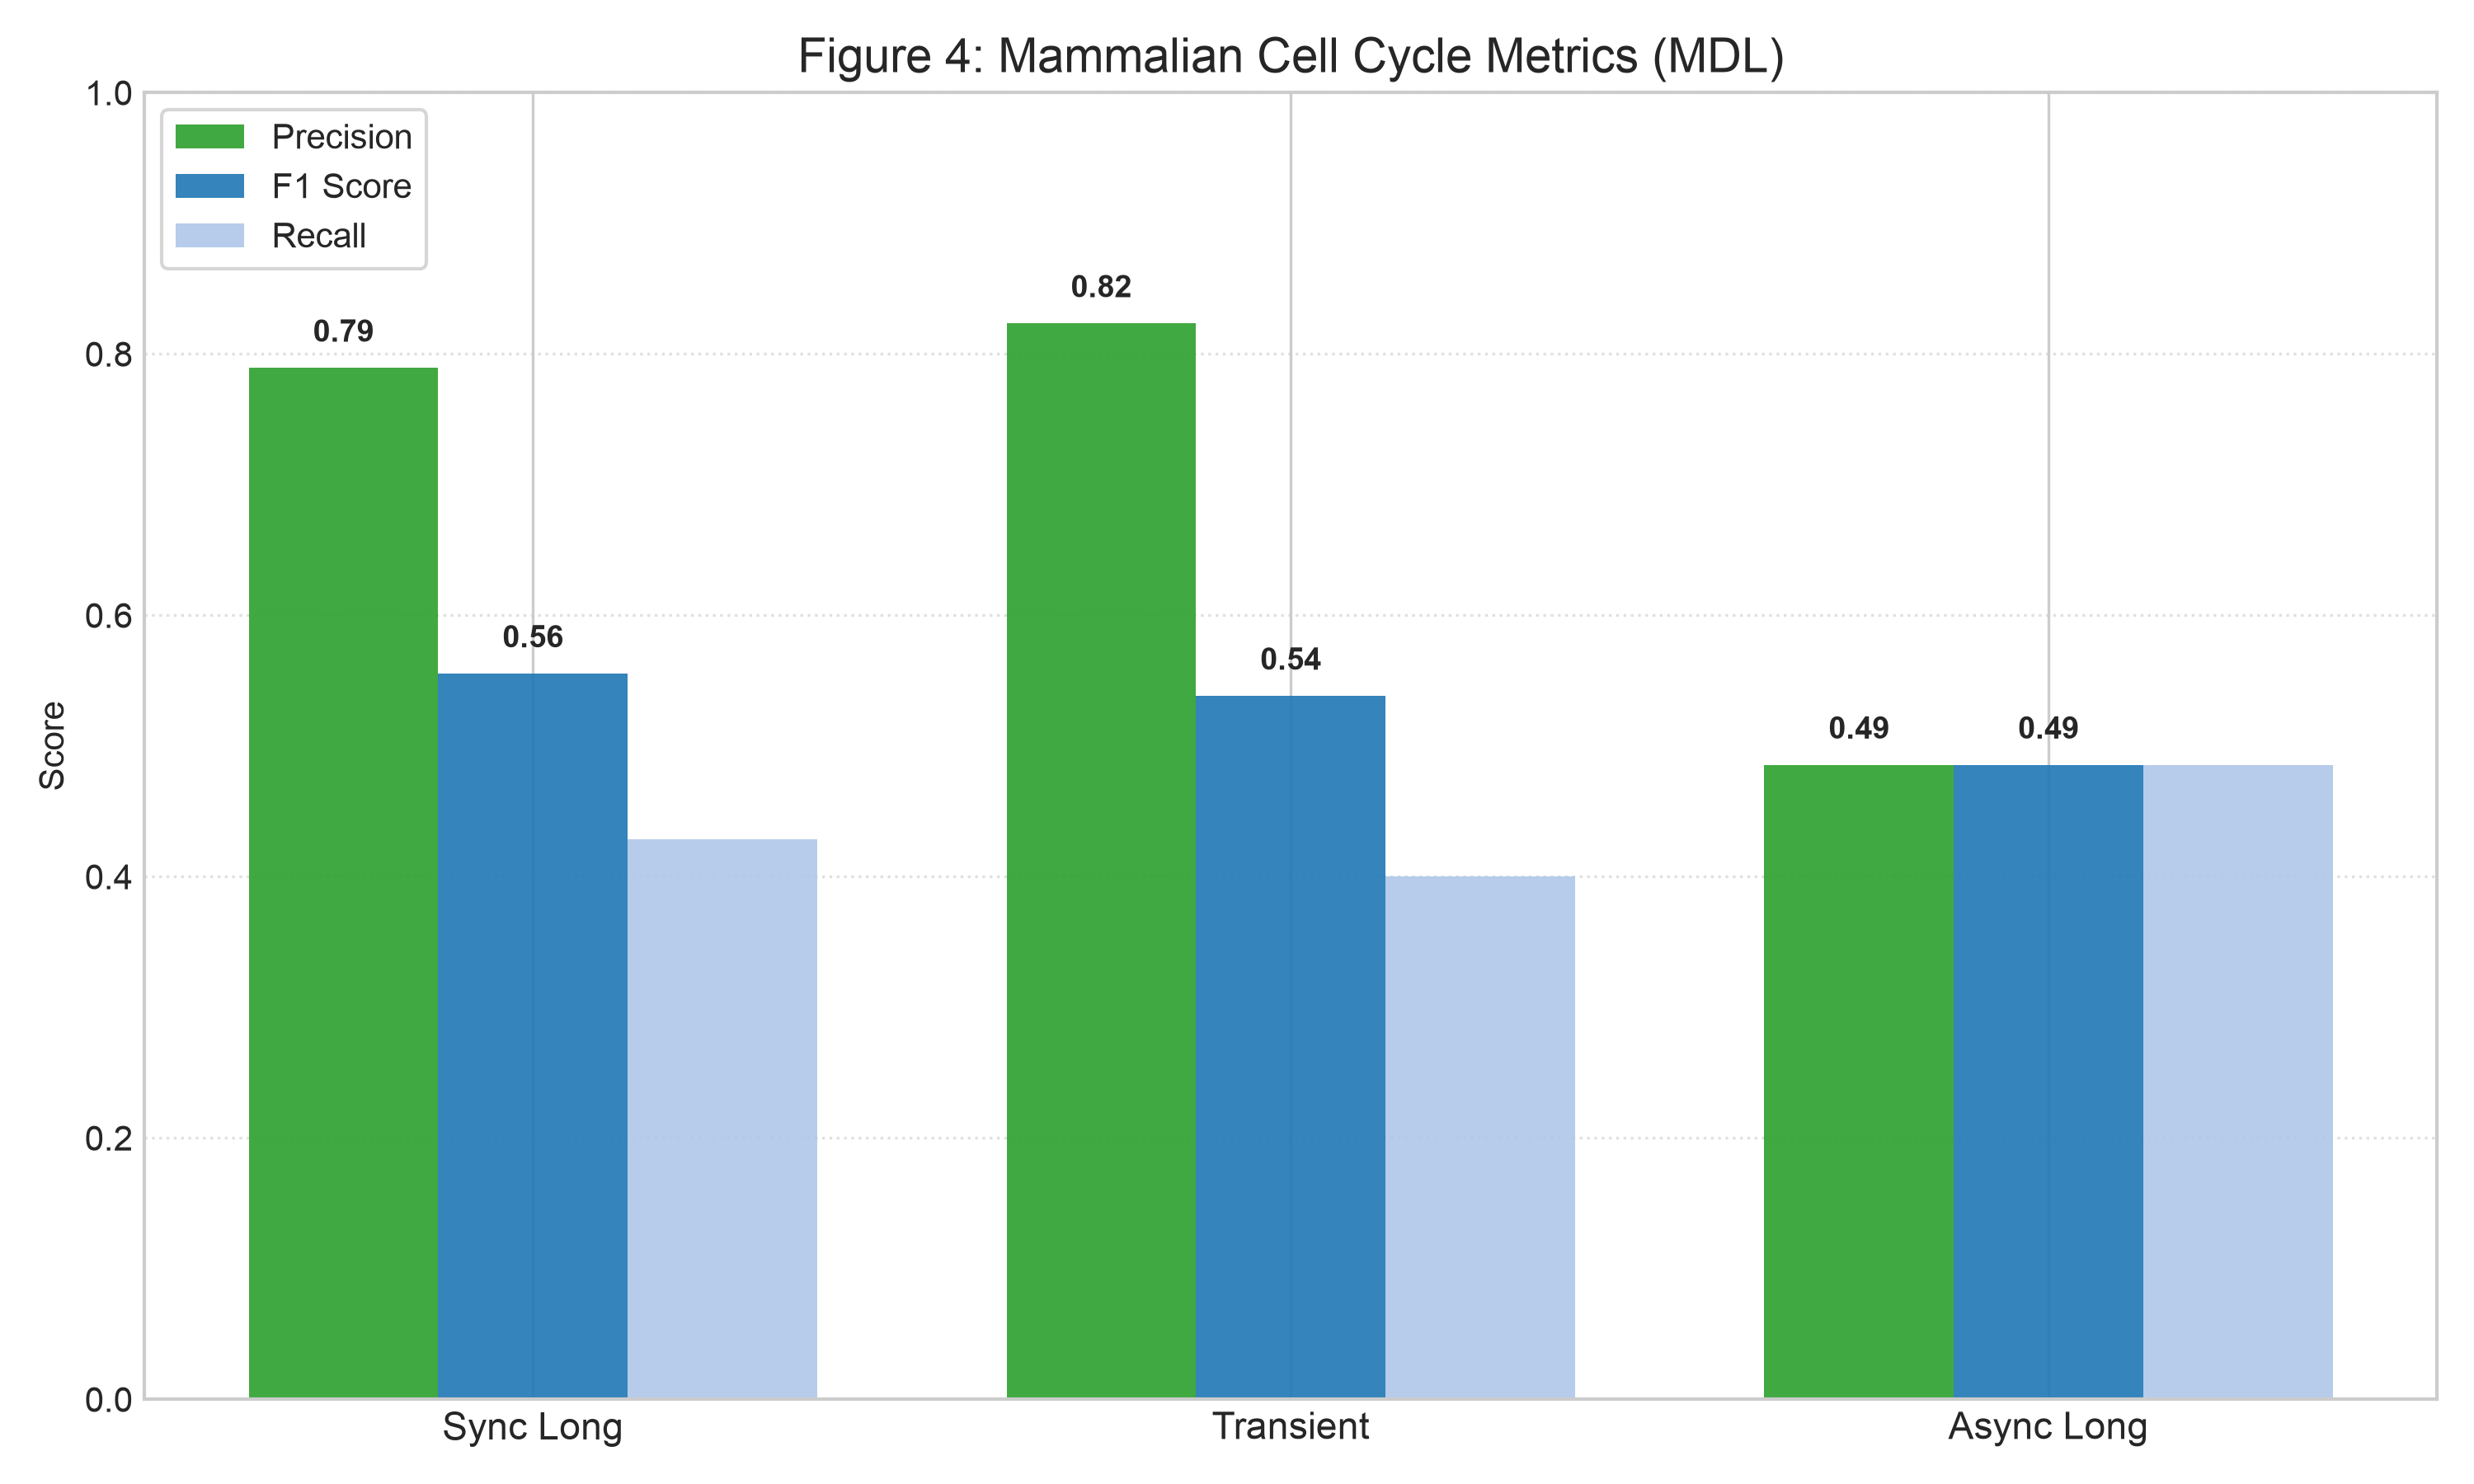
\includegraphics[width=\textwidth]{../assets/part2_metrics.png}
        \caption{MDL Performance across Regimes}
    \end{subfigure}
    \hfill
    \begin{subfigure}[b]{0.44\textwidth}
        \centering
        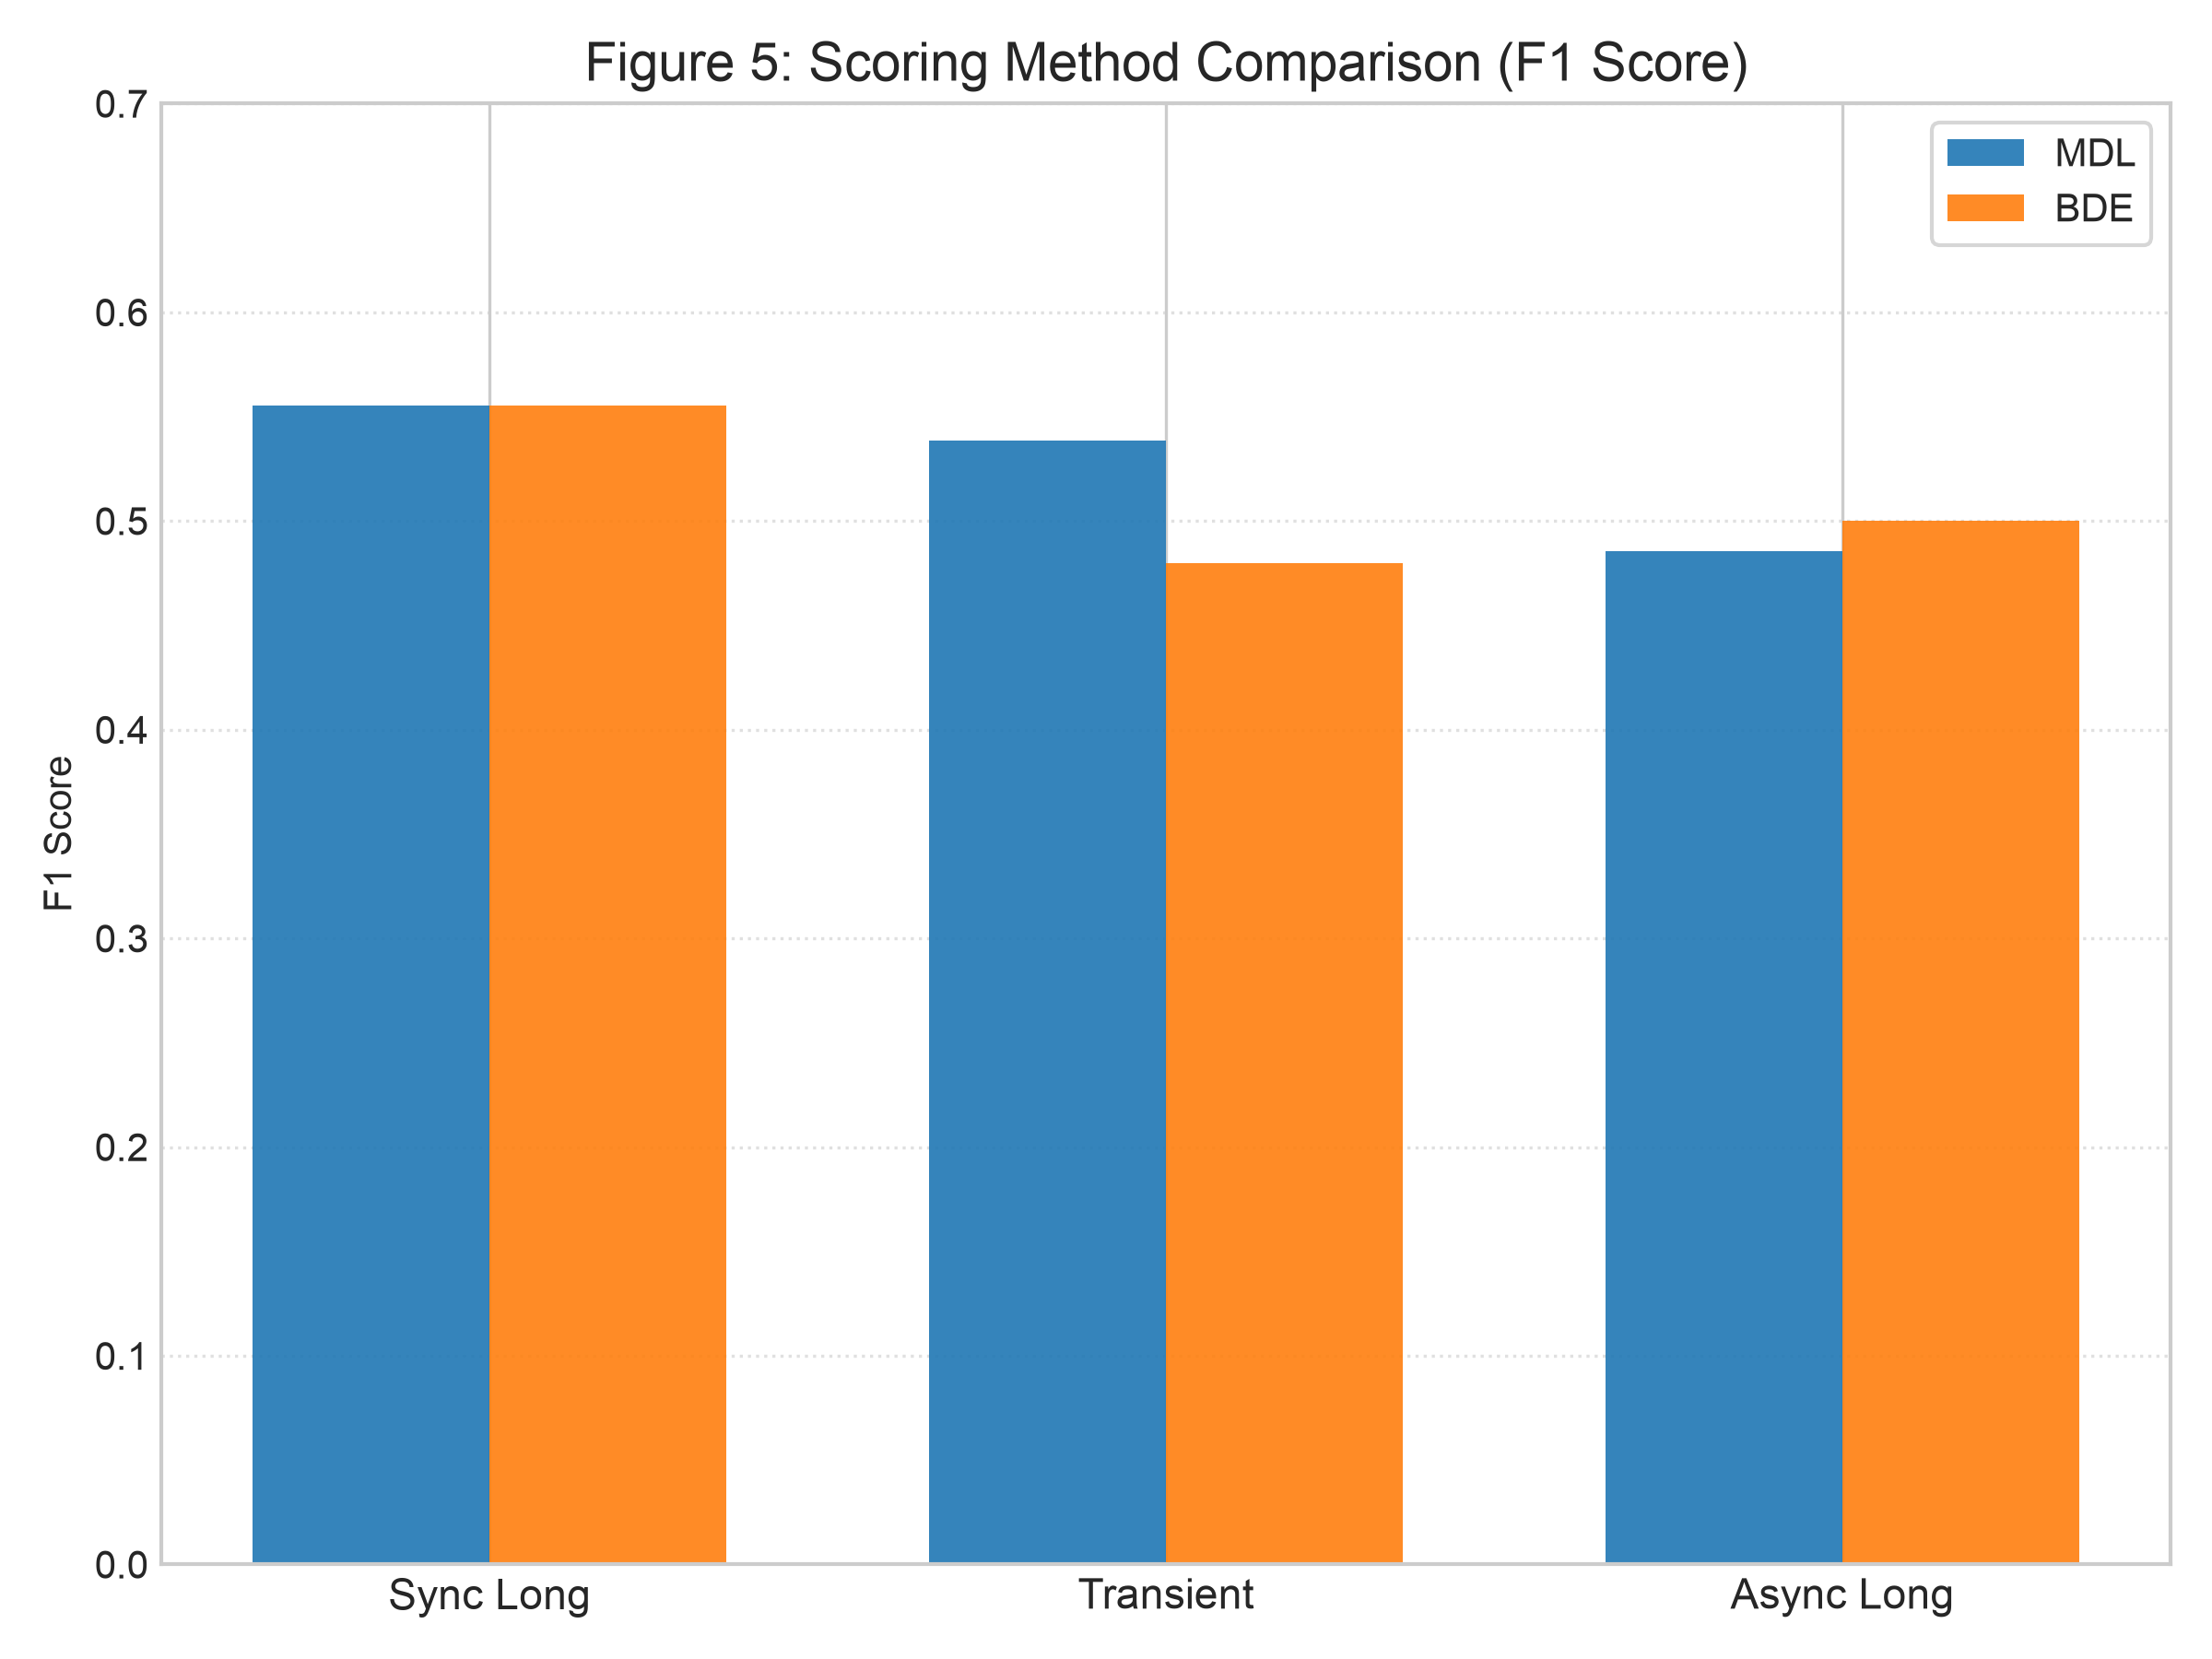
\includegraphics[width=\textwidth]{../assets/part2_method_comparison.png}
        \caption{MDL vs.\ BDE Comparison ($F_1$)}
    \end{subfigure}
    \caption{Part II: Reconstruction performance on the Mammalian Cell Cycle network.}
    \label{fig:p2}
\end{figure}

\subsection{Discussion of Biological Reconstruction}
\begin{enumerate}
    \item \textbf{High Precision of Transient \& Synchronous Regimes:} On the biological network, \texttt{transient\_bursts} paired with MDL achieved the highest Precision ($0.82$) and tied with \texttt{sync\_long} ($F_1 = 0.56, \text{Precision} = 0.79$) for the lowest Structural Hamming Distance ($\text{SHD} = 24$). Moreover, reconstruction on the 10-node biological network ($F_1 = 0.56$) substantially outperformed the 10-node synthetic RBN ($F_1 = 0.41$ for \texttt{sync\_base}, $0.07$ for \texttt{async}).
    \item \textbf{Precision--Recall Trade-off in Asynchronous Data:} The \texttt{async\_long} regime achieved the highest Recall ($0.49$ with MDL, $0.60$ with BDE) by perturbing individual nodes out of synchronous lockstep, but suffered from false-positive edges ($\text{Precision} = 0.43 - 0.49$, $\text{SHD} = 36 - 42$).
    \item \textbf{MDL vs.\ BDE:} MDL consistently matched or outperformed BDE in structural accuracy ($\text{SHD} = 24$ vs.\ $26$ in transient; $\text{SHD} = 36$ vs.\ $42$ in async) by penalizing spurious parent sets.
\end{enumerate}

\section{Conclusions}
\begin{enumerate}
    \item \textbf{Precision via Transient \& Synchronous Perturbations:} Multi-replicate synchronous and transient trajectories yield the highest precision ($0.79 - 0.82$) and lowest structural edit distance ($\text{SHD} = 24$), making them reliable for biological hypothesis generation.
    \item \textbf{Temporal Resolution Sensitivity:} Sub-sampling ($\Delta t = 3$) destroys first-order Markov transition signals ($F_1 = 0.00$ across $N \le 13$); high sampling frequency over short bursts is strictly preferable to sparse long-horizon monitoring.
    \item \textbf{Parsimony in Structure Scoring:} MDL regularization effectively suppresses false-positive edges compared to BDE, particularly under short transient bursts and stochastic asynchronous updates.
\end{enumerate}

\end{document}